% When using TeXShop on the Mac, let it know the root document. The following
% must be one of the first 20 lines.
% !TEX root = ../design.tex

% Licensed to the Apache Software Foundation (ASF) under one
% or more contributor license agreements.  See the NOTICE file
% distributed with this work for additional information
% regarding copyright ownership.  The ASF licenses this file
% to you under the Apache License, Version 2.0 (the
% "License"); you may not use this file except in compliance
% with the License.  You may obtain a copy of the License at

%   http://www.apache.org/licenses/LICENSE-2.0

% Unless required by applicable law or agreed to in writing,
% software distributed under the License is distributed on an
% "AS IS" BASIS, WITHOUT WARRANTIES OR CONDITIONS OF ANY
% KIND, either express or implied.  See the License for the
% specific language governing permissions and limitations
% under the License.

\chapter[Graph]{Graph}

\begin{moduleinfo}
\item[Authors] \href{mailto:okislal@pivotal.io}{Orhan Kislal}, \href{mailto:njayaram@pivotal.io}{Nandish Jayaram},
			   \href{mailto:rraghu@pivotal.io}{Rashmi Raghu}, \href{mailto:jmei@pivotal.io@pivotal.io}{Jingyi Mei},
			   \href{mailto:nkak@pivotal.io}{Nikhil Kak}
\item[History]
	\begin{modulehistory}
		\item[v0.1] Initial version, SSSP only.
		\item[v0.2] Graph Framework, SSSP implementation details.
        \item[v0.3] PageRank
        \item[v0.4] APSP
        \item[v0.5] Weakly Connected Components
        \item[v0.6] Breadth First Search (BFS)
        \item[v0.7] Hyperlink-Induced Topic Search (HITS)
	\end{modulehistory}
\end{moduleinfo}


% Abstract. What is the problem we want to solve?

This module implements various graph algorithms that are used in a number of
applications such as social networks, telecommunications and road networks.

\section{Graph Framework} \label{sec:graph:fw}

MADlib graph representation depends on two structures, a \emph{vertex} table
and an \emph{edge} table. The vertex table has to have a column of vertex ids.
The edge table has to have 2 columns: source vertex id, destination vertex id.
For most algorithms an edge weight column is required as well. The
representation assumes a directed graph, an edge from $x$ to $y$ does
\emph{not} guarantee the existence of an edge from $y$ to $x$. Both of the
tables may have additional columns as required. Multi-edges (multiple edges
from a vertex to the same destination) and loops (edge from a vertex to
itself) are allowed. This representation does not impose any ordering of
vertices or edges. An example graph is given in Figure~\ref{sssp:example} and
its representative tables are given in Table~\ref{sssp:rep}.

\begin{figure}[h]
	\centering
	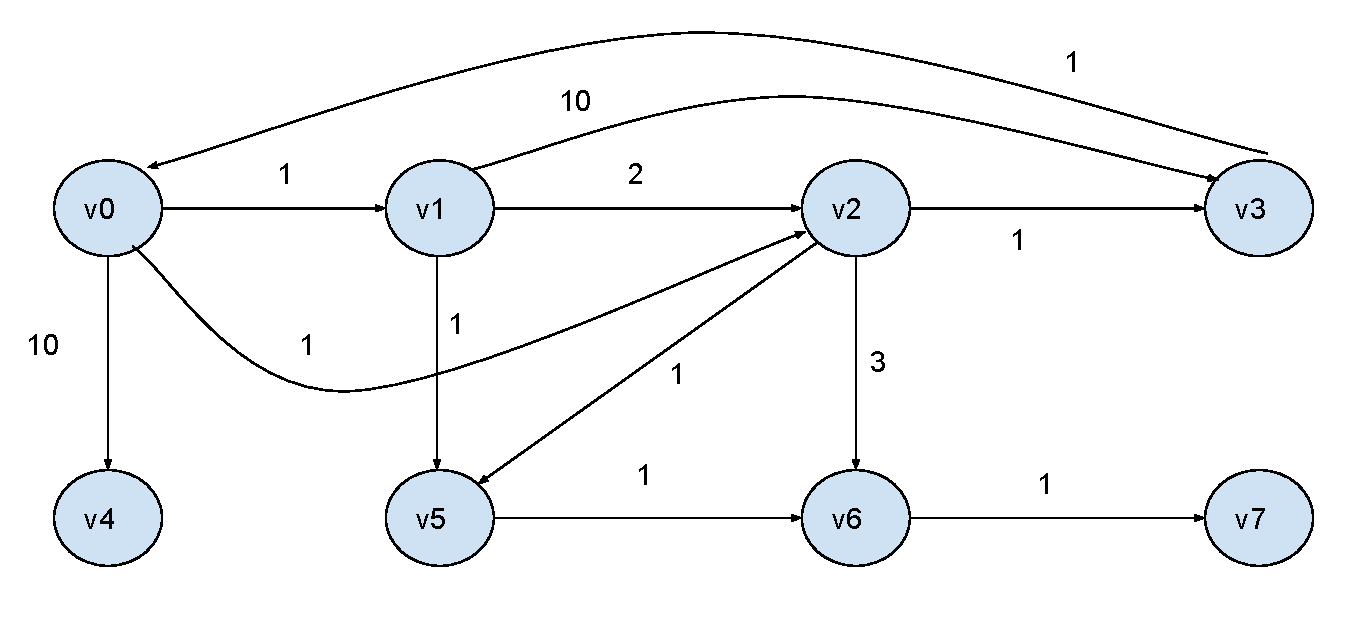
\includegraphics[width=0.9\textwidth]{figures/graph_example.pdf}
\caption{A sample graph}
\label{sssp:example}
\end{figure}

\begin{table}
  \begin{tabular}{| c | }
    \hline
    vid \\ \hline
    0 \\ \hline
    1 \\ \hline
    2 \\ \hline
    3 \\ \hline
    4 \\ \hline
    5 \\ \hline
    6 \\ \hline
    7 \\
    \hline
  \end{tabular}
  \quad
  \begin{tabular}{| c | c | c |}
    \hline
    src & dest & weight \\ \hline
    0 & 1 & 1 \\ \hline
    0 & 2 & 1 \\ \hline
    0 & 4 & 10 \\ \hline
    1 & 2 & 2 \\ \hline
    1 & 3 & 10 \\ \hline
    1 & 5 & 1 \\ \hline
    2 & 3 & 1 \\ \hline
    2 & 5 & 1 \\ \hline
    2 & 6 & 3 \\ \hline
    3 & 0 & 1 \\ \hline
    5 & 6 & 1 \\ \hline
    6 & 7 & 1 \\
    \hline
  \end{tabular}
  \caption{Graph representation of vertices (left) and edges(right) in the
  database}
  \label{sssp:rep}
\end{table}


\section{Single Source Shortest Path} \label{sec:graph:sssp}

Given a graph and a source vertex, single source shortest path (SSSP)
algorithm finds a path for every vertex such that the sum of the weights of
its constituent edges is minimized.

Shortest path is defined as follows. Let $e_{i,j}$ be the edge from vertex $i$
to vertex $j$ and $w_{i,j}$ be its weight. Given a graph G, the shortest path
from $s$ to $d$ is $P = (v_1, v_2 \dots, v_n)$ (where $v_1=s$ and $v_n=d$)
that over all possible $n$ minimizes the sum $ \sum _{i=1}^{n-1}f(e_{i,i+1})$.

% \subsection{Bellman Ford Algorithm}

Bellman-Ford Algorithm \cite{bellman1958routing,ford1956network} is based on
the following idea: We start with a naive approximation for the cost of
reaching every vertex. At each iteration, these values are refined based on
the edge list and the existing approximations. If there are no refinements at
any given step, the algorithm returns the calculated results. If the algorithm
does not converge in $|V|-1$ iterations, this indicates the existence of a
negative cycle in the graph.


\begin{algorithm}[SSSP$(V,E,start)$] \label{alg:sssp}
\alginput{Vertex set $V$, edge set $E$, starting vertex $start$}
\algoutput{Distance and parent set for every vertex $cur$}
\begin{algorithmic}[1]
	\State $toupdate(0) \set (start,0,start)$
	\For{every $i \in 0\dots|V|-1$}
		\For{every tuple $t \in toupdate(i)$} \label{alg:sssp:update}
			\For{every edge $e \mid e.src = t.id$}
		 		\State $local \set e.val + t.val$
		 		\If{$local < toupdate(i+1,e.dest).val$} \label{alg:sssp:single}
		 			\State $toupdate(i+1,dest) \set (local,e.src)$
		 		\EndIf
			\EndFor
		\EndFor
		\For{every tuple $t \in toupdate(i+1)$}
		 	\If{$t.val < cur(t.id).val$}
		 		\State $cur(t.id) \set (t.val,t.parent)$
		 	\EndIf
		\EndFor
	\EndFor
\end{algorithmic}
\end{algorithm}

\begin{description}
\item edge: $(src,dest,val)$. The edges of the graph.
\item cur: $id \rightarrow (val,parent)$. The intermediate SSSP results.
\item toupdate: $iter \rightarrow (id \rightarrow (val,parent))$. The set of updates.
\end{description}

Changes from the standard Bellman-Ford algorithm:

\begin{description}
\item Line~\ref{alg:sssp:update}: We only check the vertices that have been
updated in the last iteration.
\item Line~\ref{alg:sssp:single}: At each iteration, we update a given vertex
only one time. This means the toupdate set cannot contain multiple records
for the same vertex which requires the comparison with the existing value.
\end{description}

This is not a 1-to-1 pseudocode for the implementation since we don't compare
the `toupdate` table records one by one but calculate the overall minimum. In
addition, the comparison with `cur` values take place earlier to reduce the
number of tuples in the `toupdate` table.

\subsection{Implementation Details}

In this section, we discuss the MADlib implementation of the SSSP algorithm
in depth.

\begin{algorithm}[SSSP$(V,E,start)$] \label{alg:sssp:high}
\begin{algorithmic}[1]
	\Repeat
		\State Find Updates
		\State Apply updates to the output table
	\Until {There are no updates}
\end{algorithmic}
\end{algorithm}

The implementation consists of two SQL blocks that are called sequentially
inside a loop. We will follow the example graph at Figure~\ref{sssp:example}
with the starting point as $v_0$. The very first update on the output table is
the source vertex. Its weight is $0$ and its parent is itself ($v_0$). After
this initialization step, the loop starts with Find Updates (the individual
updates will be represented with <dest,value,parent> format). Looking at the
example, it is clear that the updates should be <1,1,0>, <2,1,0> and <4,10,0>.
We will assume this iteration is already completed and look how the next
iteration of the algorithm works to explain the implementation details.

\begin{algorithm}[Find Updates$(E,old\_update,out\_table)$]
\label{alg:sssp:findu}
\begin{lstlisting}
INSERT INTO new_update
	SELECT DISTINCT ON (y.id) y.id AS id,
		y.val AS val,
		y.parent AS parent
	FROM out_table INNER JOIN (
			SELECT edge_table.dest AS id, x.val AS val, old_update.id AS parent
			FROM old_update
				INNER JOIN edge_table
				ON (edge_table.src = old_update.id)
				INNER JOIN (
					SELECT edge_table.dest AS id,
						min(old_update.val + edge_table.weight) AS val
					FROM old_update INNER JOIN
						edge_table AS edge_table ON
						(edge_table.src=old_update.id)
					GROUP BY edge_table.dest
				) x
				ON (edge_table.dest = x.id)
			WHERE ABS(old_update.val + edge_table.weight - x.val) < EPSILON
		) AS y ON (y.id = out_table.vertex_id)
	WHERE y.val<out_table.weight
\end{lstlisting}
\end{algorithm}

The Find Updates query is constructed in 4 levels of subqueries: \emph{find
values, find parents, eliminate duplicates and ensure improvement}.

\begin{itemize}

\item We begin our analysis at the innermost subquery, emph{find values}
(lines 11-16). This subquery takes a set of vertices (in the table
$old\_update$) and finds the reachable vertices. In case a vertex is reachable
by multiple vertices, only the path that has the minimum cost is considered
(hence the name find values). There are two important points to note:
	\begin{itemize}
	\item The input vertices need the value of their path as well.
		\begin{itemize}
		\item In our example, both $v_1$ and $v_2$ can reach $v_3$. We would
		have to use $v_2 \rightarrow v_3$ edge since that gives the lowest possible
		path value.
		\end{itemize}
	\item The subquery is aggregating the rows using the $min$ operator for
	each destination vertex and  unable to return the source vertex at the
	same time to use as the parent value.
		\begin{itemize}
		\item We know the value of $v_3$ should be $2$ but we cannot know
		its parent ($v_2$) at the same time.
		\end{itemize}
	\end{itemize}

\item The \emph{find parents} subquery is designed to solve the
aforementioned limitation. We combine the result of \emph{find values} with
$edge$ and $old\_update$ tables (lines 7-10) and get the rows that has the
same minimum value.
	\begin{itemize}
	\item Note that, we would have to tackle the problem of tie-breaking.
		\begin{itemize}
		\item Vertex $v_5$ has two paths leading into: <5,2,1> and <5,2,2>.
		The inner subquery will return <5,2> and it will match both of these
		edges.
		\end{itemize}
	\item It is redundant to keep both of them in the update list as that
	would require updating the same vertex multiple times in a given
	iteration.
	\end{itemize}

\item At this level, we employ the \emph{eliminate duplicates} subquery. By
using the $DISTINCT$ clause at line 2, we allow the underlying system to
accept only a single one of them.

\item Finally, we introduce the \emph{ensure improvement} subquery to make
sure these updates are actually leading us to shortest paths. Line 21 ensures
that the values stored in the $out\_table$ does not increase and the solution
does not regress throughout the iterations.
\end{itemize}

Applying updates is straightforward as the values and the associated parent
values are replaced using the $new\_update$ table. After this operation is
completed the $new\_update$ table becomes $old\_update$ for the next iteration
of the algorithm.

Please note that, for ideal performance, \emph{vertex} and \emph{edge} tables
should be distributed on \emph{vertex id} and \emph{source id} respectively.

\section{All Pairs Shortest Paths} \label{sec:graph:apsp}

Given a graph and a source vertex, all pairs shortest paths (APSP) algorithm
finds a path for every vertex pair such that the sum of the weights of its
constituent edges is minimized. Please refer to the
Section~\ref{sec:graph:sssp} on single source shortest path for the
mathematical definition of shortest path.

Our implementation has a dynamic programming approach, based on the matrix
multiplication inspired APSP algorithm \cite{apsp}. The idea is similar to
the one from SSSP implementation. We start with a naive approximation for the
cost of every vertex pair (infinite). At each iteration, these values are
refined based on the edge list and the existing approximations. This
refinement step is similar to a matrix multiplication. For every vertex pair
$i,j$, we check every edge $e: j \rightarrow k$ to see if it is possible to
use $e$ to reduce the cost of path $i \rightarrow k$. If there are no
refinements at any given step, the algorithm returns the calculated results.
If the algorithm does not converge in $|V|-1$ iterations, this indicates the
existence of a negative cycle in the graph.

\begin{algorithm}[APSP$(V,E)$] \label{alg:apsp}
\alginput{Vertex set $v$, edge set $E$}
\algoutput{Distance and parent set for every vertex pair}
\begin{algorithmic}[1]

	\While {$update$ is $True$}
		\State $update \set False$
		\For{every vertex pair $i,j$}
			\For{every edge $j \rightarrow k$}
		 		\If{$ val(i \rightarrow j) + val(j \rightarrow k) < val(i \rightarrow k)$}
		 			\State $val(i \rightarrow k) \set  val(i \rightarrow j) + val(j \rightarrow k)$
		 			\State $parent(i \rightarrow k) \set j$
		 			\State $update \set True$
		 		\EndIf
			\EndFor
		\EndFor
	\EndWhile
\end{algorithmic}
\end{algorithm}

\subsection{Implementation Details}

The implementation details are similar to the SSSP as the requirements and
restrictions such as finding the parent, distinct updates, etc. are common in
both cases. This section will mostly focus on the differences in the APSP
implementation.

\begin{algorithm}[Find Updates$(E,out)$]
\label{alg:apsp:findu}
\begin{lstlisting}
INSERT INTO update
	SELECT DISTINCT ON (y.src, y.dest) y.src AS src, y.dest AS dest
		y.val AS val,
		y.parent AS parent
	FROM out INNER JOIN (
			SELECT
				x.src AS src, x.dest AS dest,
				x.val AS val, out.dest AS parent
			FROM out
				INNER JOIN edge_table
				ON (edge_table.src = out.dest)
				INNER JOIN (
					SELECT out.src AS src, edge_table.dest AS dest,
						min(out.val + edge_table.weight) AS val
					FROM out INNER JOIN
						edge_table ON
						(edge_table.src=out.dest)
					GROUP BY out.src, edge_table.dest
				) x
				ON (edge_table.src = x.src AND edge_table.dest = x.dest)
			WHERE ABS(out.val + edge_table.weight - x.val) < EPSILON
		) AS y ON (y.src = out.src AND y.dest = out.dest)
	WHERE y.val < out.val
\end{lstlisting}
\end{algorithm}

The only major difference comes in the innermost subquery (lines 13-18). The
\emph{group by} clause ensures that we try to reduce the weight for every
$out.src$ ($i$) and $edge\_table.dest$ ($k$) pair. The \emph{inner join on}
clause ensures that there is a connecting edge ($j\rightarrow k$) that can be
used for the $i,j$ pair. The rest of the changes are mostly trivial as the
algorithm needs to check for both source and destination during joins (instead
of just the destination).


\section{PageRank} \label{sec:graph:pagerank}
\begin{figure}[h]
    \centering
    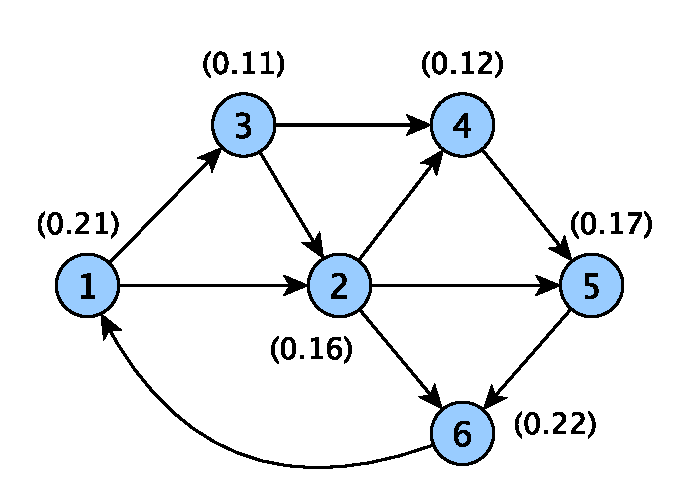
\includegraphics[width=0.5\textwidth]{figures/pagerank_example.pdf}
\caption{An example graph for PageRank}
\label{pagerank:example}
\end{figure}

PageRank is a link analysis algorithm that assigns a score to every vertex
measuring the relative importance of vertices within the set of all
vertices. PageRank~\cite{pagerank} was first used by Google to measure the
importance of website pages where the World Wide Web was modeled as a directed
graph. Figure~\ref{pagerank:example} shows an example graph with the PageRank
value of each vertex. The intuition behind the algorithm is that the number and
quality of links to a vertex determine the authoritativeness of the vertex,
which is reflected in the PageRank scores as shown in the figure.

The pagerank module in MADlib implements the model of a random surfer who
follows the edges of a graph to traverse it, and jumps to a random vertex
after several clicks. The random surfer is modeled using a damping factor
that represents the probability with which the surfer will continue to follow
links in the graph rather than jumping to a random vertex. MADlib's pagerank
module outputs a probability distribution that represents the likelihood that
the random surfer arrives at a particular vertex in the graph.

PageRank is an iterative algorithm where the PageRank scores of vertices from
the previous iteration are used to compute the new PageRank scores. The
PageRank score of a vertex $v$, at the $i^{th}$ iteration, denoted by $PR(v_i)$
is computed as:

\begin{equation}
PR(v_i) = \frac{1-d}{N} + d \sum_{u \in M(v)}(\frac{PR(u_{i-1})}{L(u)})
\label{eq:pagerank}
\end{equation}

where $N$ is the number of vertices in the graph, $d$ is the damping factor,
$M(v)$ represents the set of vertices that have an edge to vertex $v$,
$L(u)$ represents the out-degree of vertex $u$, i.e., the number of
out-going edges from vertex $u$, and $PR(u_{i-1})$ represents the PageRank
score of vertex $u$ in the $(i-1)^{st}$ iteration.

$\frac{1-d}{N}$ represents the tiny probability with which the surfer
would randomly jump to vertex $v$, rather than arriving at $v$ following
links in the graph. This ensures that there is some probability of visiting
every vertex in the graph even if they do not have any incoming edges. Note
that the PageRank score computed for a vertex $v$ using~\ref{eq:pagerank}
in the $i^{th}$ iteration is not updated until the new score is computed for
all the vertices in the graph. The computation terminates either when the
PageRank score of no vertex changes beyond a threshold across two consecutive
iterations, or when a pre-set number of iterations are completed.

\paragraph{Personalized Pagerank:}
The Personalized Pagerank variant of Pagerank module in MADlib takes an extra argument as a set of user provided vertices.
These personalization vertices will have a higher jump probability as compared to other vertices and random surfer is more likely to jump on these personalization vertices. These personalization vertices are initialized with an initial probabilty of $\frac{1}{N}$ where $N$ is the total number of personlaized vertices in the graph and rest of the vertices in the graph are assigned an initial probability of 0. Pagerank calculated for these vertices is biased as a random jump probability is assigned to only these vertices during the pagerank calculation,which is equal to (1 - damping factor).

\subsection{Implementation Details} \label{sec:pagerank:implementation}

In this section, we discuss the MADlib implementation of PageRank in depth.
We maintain two tables at every iteration: $previous$ and $cur$. The
$previous$ table maintains the PageRank scores of all vertices computed in
the previous iteration, while $cur$ maintains the updated scores of all
vertices in the current iteration.

\begin{algorithm}[PageRank$(V,E)$] \label{alg:pagerank:high}
\begin{algorithmic}[1]
    \State Create $previous$ table with a default PageRank score of
            $\frac{1}{N}$ for every vertex
    \Repeat
        \State Create empty table $cur$.
        \State Update $cur$ using PageRank scores of vertices in $previous$
        \State Update PageRank scores of vertices without incoming edges
        \State Drop $previous$ and rename $cur$ to $previous$
    \Until {PageRank scores have converged or \emph{max} iterations have elapsed}
\end{algorithmic}
\end{algorithm}

The implementation consists of updating the PageRank scores of all vertices
at every iteration, using the PageRank scores of vertices from the previous
iteration. The PageRank score of every vertex is initialized to $\frac{1}{N}$
where $N$ is the total number of vertices in the graph. The out-degree of
every vertex in the graph (represented by $L(u)$ in eq.~\ref{eq:pagerank}),
is captured in table $out\_cnts$. The following query is used to create and
update the PageRank scores in $cur$ table using the PageRank scores in
$previous$ table.

\begin{algorithm}[Update PageRank scores$(previous,out\_cnts,d,N)$]
\label{alg:pagerank:update}
\begin{lstlisting}
CREATE TABLE cur AS
    SELECT edge_table.dest AS id,
        SUM(previous1.pagerank/out_cnts.cnt)*d + (1-d)/N AS pagerank
    FROM edge_table
        INNER JOIN previous ON edge_table.dest = previous.id
        INNER JOIN out_cnts ON edge_table.src = out_cnts.id
        INNER JOIN previous AS previous1 ON edge_table.src = previous1.id
    GROUP BY edge_table.dest

-- Update PageRank scores of vertices without any incoming edges:
INSERT INTO cur
    SELECT id, (1-d)/N AS pagerank
    FROM previous
    WHERE id NOT IN (
        SELECT id
        FROM cur
    )
\end{lstlisting}
\end{algorithm}

The PageRank computation is terminated either when a fixed number of iterations
are completed, or when the PageRank scores of all vertices have converged. The
PageRank score of a vertex is deemed converged if the absolute difference in
its PageRank scores from $previous$ and $cur$ is less than a specified threshold.
The following query is used to find all the vertices whose PageRank scores have
not converged yet.

\begin{algorithm}[Update PageRank scores$(previous,cur,threshold)$]
\label{alg:pagerank:update}
\begin{lstlisting}
SELECT id
FROM cur
INNER JOIN previous ON cur.id = previous.id
WHERE ABS(previous.pagerank - cur.pagerank) > threshold
\end{lstlisting}
\end{algorithm}

\subsection{Best Practices} \label{sec:pagerank:bestpractices}

The pagerank module in MADlib has a few optional parameters: damping factor
$d$, number of iterations $max$, and the threshold for convergence $threshold$.
The default values for these parameters when not specified by the user are
$0.85$, $100$ and $\frac{1}{N*1000}$ respectively.

The damping factor denotes the probability with which the surfer uses the edges
to traverse the graph. If set to $0$, it implies that the only way a surfer
would visit a vertex in the graph is by randomly jumping to it. If set to
$1$, it implies that the only way the surfer can reach a vertex is by following
the edges in the graph, thus precluding the surfer from reaching a vertex
that has no incoming edges. It is common practice to set damping factor
to $0.85$~\cite{pagerank}, and the maximum number of iterations to $100$.
The convergence test for PageRank in MADlib checks for the delta between
the PageRank scores of a vertex across two consecutive iterations. Since
the initial value of the PageRank score is set to $\frac{1}{N}$, the delta
will be small in the initial iterations when $N$ is large (say over 100
million). We thus set the threshold to $\frac{1}{N*1000}$, and it is to be
noted that this is not based on any experimental study. Users of MADlib are
encouraged to consider this factor when setting a value for threshold, since
a high $threshold$ value would lead to early termination of PageRank
computation, thus resulting in incorrect PageRank values.


\section{Weakly Connected Components} \label{sec:graph:wcc}
\begin{figure}[h]
    \centering
    \includegraphics[width=0.5\textwidth]{figures/wcc_example.pdf}
\caption{An example disconnected directed graph}
\label{wcc:example}
\end{figure}

Given a directed graph $G$, a weakly connected component is a subgraph
$G_{sub}$ of $G$, such that there exists a path from every vertex in $G_{sub}$
to every other vertex in $G_{sub}$, ignoring the direction of the edges.

The weakly connected component module implemented in MADlib is based on
GRAIL~\cite{grail}. All vertices are initialized with their own vertex
ID as the component ID, and are considered to be active. In every iteration,
each active vertex's component ID is updated with the smallest component ID
value of all its neighbors. Any vertex whose component ID is not updated in
the current iteration is deemed as an inactive vertex for the next iteration.
Execution continues until there are no active vertices left. Since each vertex
is initialized with its own ID as the component ID, and updated based on
neighboring nodes' component IDs, the final component ID of a component will
be equal to the smallest vertex ID in the corresponding subgraph.
Figure~\ref{wcc:example} shows an example directed graph with two disconnected
subgraphs. The subgraph containing vertices $1$, $2$, $3$, $4$, $5$ and $6$
forms a weakly connected component, and is assigned component ID 1, while the
subgraph containing vertices $12$, $14$, $21$ and $23$ forms the second component
and is assigned component ID 12.

\subsection{Implementation Details} \label{sec:wcc:implementation}

In this section, we discuss the MADlib implementation of weakly connected
components in depth. We maintain the following tables at every iteration:
$oldupdate$, $message$ and $newupdate$. In $newupdate$, the component ID
of each vertex is initialized to infinity, while the component ID of vertices
in the $message$ table is initialized to their corresponding vertex ID.

\begin{algorithm}[Weakly Connected Components$(V,E)$] \label{alg:wcc:high}
\begin{algorithmic}[1]
    \State Create $newupdate$ table with a default component ID of
            $infinity$ for every vertex
    \State Create $message$ table with a default component ID of the
            corresponding $id$ (vertex ID) for every vertex
    \Repeat
        \State Update the $oldupdate$ table
        \State Update $toupdate$ table with active vertices
        \State Update the $newupdate$ table
        \State Update $message$ table with potential new component IDs for each vertex
    \Until {There are no active vertices in $toupdate$ table}
\end{algorithmic}
\end{algorithm}

The $message$ table contains the component IDs associated with all its
immediate neighbors. At each iteration, $oldupdate$ is updated with the
minimum of all the associated component IDs found for a vertex in $message$.

\begin{algorithm}[Update oldupdate table]
\begin{lstlisting}
SELECT id, MIN(message.component_id) as component_id
FROM message
GROUP BY id
\end{lstlisting}
\end{algorithm}

Table $toupdate$ records all vertices whose component IDs must be updated,
and are thus marked active.

\begin{algorithm}[Update toupdate table with active vertices]
\begin{lstlisting}
-- Find vertices whose component ID must be updated
CREATE TABLE toupdate AS
SELECT id, component_id
FROM oldupdate, newupdate
WHERE oldupdate.id = newupdate.id AND
        oldupdate.component_id < newupdate.component_id

-- Update the component IDs
UPDATE newupdate SET
component_id = toupdate.component_id
FROM toupdate
WHERE newupdate.id = toupdate.id
\end{lstlisting}
\end{algorithm}

Finally, the $message$ table is updated with potential new
component IDs for active vertices using the following query:

\begin{algorithm}[Update message table$(toupdate, edge)$]
\label{alg:wcc:message}
\begin{lstlisting}
CREATE TEMP TABLE message AS
SELECT id, MIN(component_id) AS component_id
FROM (
    SELECT edge.src AS id,
        toupdate.component_id
    FROM toupdate, edge
    WHERE edge.dest = toupdate.id
    UNION ALL
    SELECT edge.dest AS id,
        toupdate.component_id
    FROM toupdate, edge
    WHERE edge.src = toupdate.id
) AS t
GROUP BY id
\end{lstlisting}
\end{algorithm}

At the end of the computation, $newupdate$ will have the component ID
associated with each vertex in $G$. The component ID of all the vertices
in a component is equal to the smallest vertex ID in the corresponding
subgraph.

\subsection{Edge Table Duplication} \label{sec:wcc:duplication}

The queries explained in the Section~\ref{sec:wcc:implementation} expose a
potential performance drawback in Greenplum systems. In general, we advise
that the edge tables should be distributed by their source columns. However,
in WCC, we use both source and destination columns of the edge table in JOIN
clauses. In addition, we employ a GROUP BY clause using the column that did
not serve as the join key. Algorithm~\ref{alg:wcc:message} shows that when $dest$
is used for the JOIN clause, $src$ is renamed to $id$ to be used for GROUP BY
and vice versa. This query forces multiple redistribute motions in the
database which might cause performance degradation. To address this issue, we
create a duplicate of the edge table and distribute on the destination column
(only for Greenplum systems).

\section{Breadth-first Search} \label{sec:graph:bfs}

Given a graph $G$ and a user-specified origin vertex $src$, this algorithm
searches and discovers connected nodes in a graph in breadth-first order
\cite{bfs_wikipedia}. The graph can be treated as either directed or
undirected based on a parameter specified when calling the function.
There is also a parameter to control the number of hops (edges) to traverse
from the source vertex. If not specified, all nodes accessible from the
source node will be discovered.

\subsection{Implementation Details}
\begin{algorithm}[Breadth First Search$(V, E, src)$] \label{alg:bfs:high}
\begin{algorithmic}[1]
    \State Set $dist \leftarrow 0$
    \State Create $message$ table with $src$ vertex, $NULL$ parent, and $dist$
    \State Copy $message$ table to output table $out$
    \Repeat
        \State Create $toupdate$ table using $out$ and $message$ tables
        \State $dist \leftarrow dist + 1$
        \State Update $message$ table with newly found candidate vertices, parent and $dist$
        \State Copy $message$ table to $out$
    \Until {There are no candidate vertices remaining in $message$ table}
\end{algorithmic}
\end{algorithm}

The implementation details are similar to SSSP, albeit simpler. We only have to
track the number of hops and not the sum of weights, but other requirements and
restrictions such as finding the parent, distinct updates, etc. are common in
both cases. The output table is initialized only to the $src$ vertex to begin
with. A $message$ table is also maintained that contains the list of vertices
to traverse and explore in the next iteration, which is also initialized with
the $src$ vertex. BFS then runs iteratively until no more candidate vertices
remain in the $message$ table, as outlined in~\ref{alg:bfs:high}.

At every iteration, $toupdate$ table is updated with vertices that are neighbors
of vertices in the $message$ table, that are not already visited in the past
(one scan of the $out$ table reveals all the vertices that have already been
visited in the past). All such newly found neighboring vertices in the current
iteration will have one or more parents, based on how many vertices in the
$message$ table have a direct edge to them. Each such vertex in the $message$
table is marked as the parent of such newly found neighboring vertices in
the $toupdate$ table.

The $message$ table is then cleared and updated with the contents of $toupdate$
table, except that for each new neighboring vertex considered, only one of the
parents is recorded as its parent (the node with the smallest id among all
parent nodes). The content of this updated $message$ is then copied
to the $out$ table, and this process continues until $message$ table is empty.


\section{HITS} \label{sec:graph:hits}
\begin{figure}[h]
	\centering
	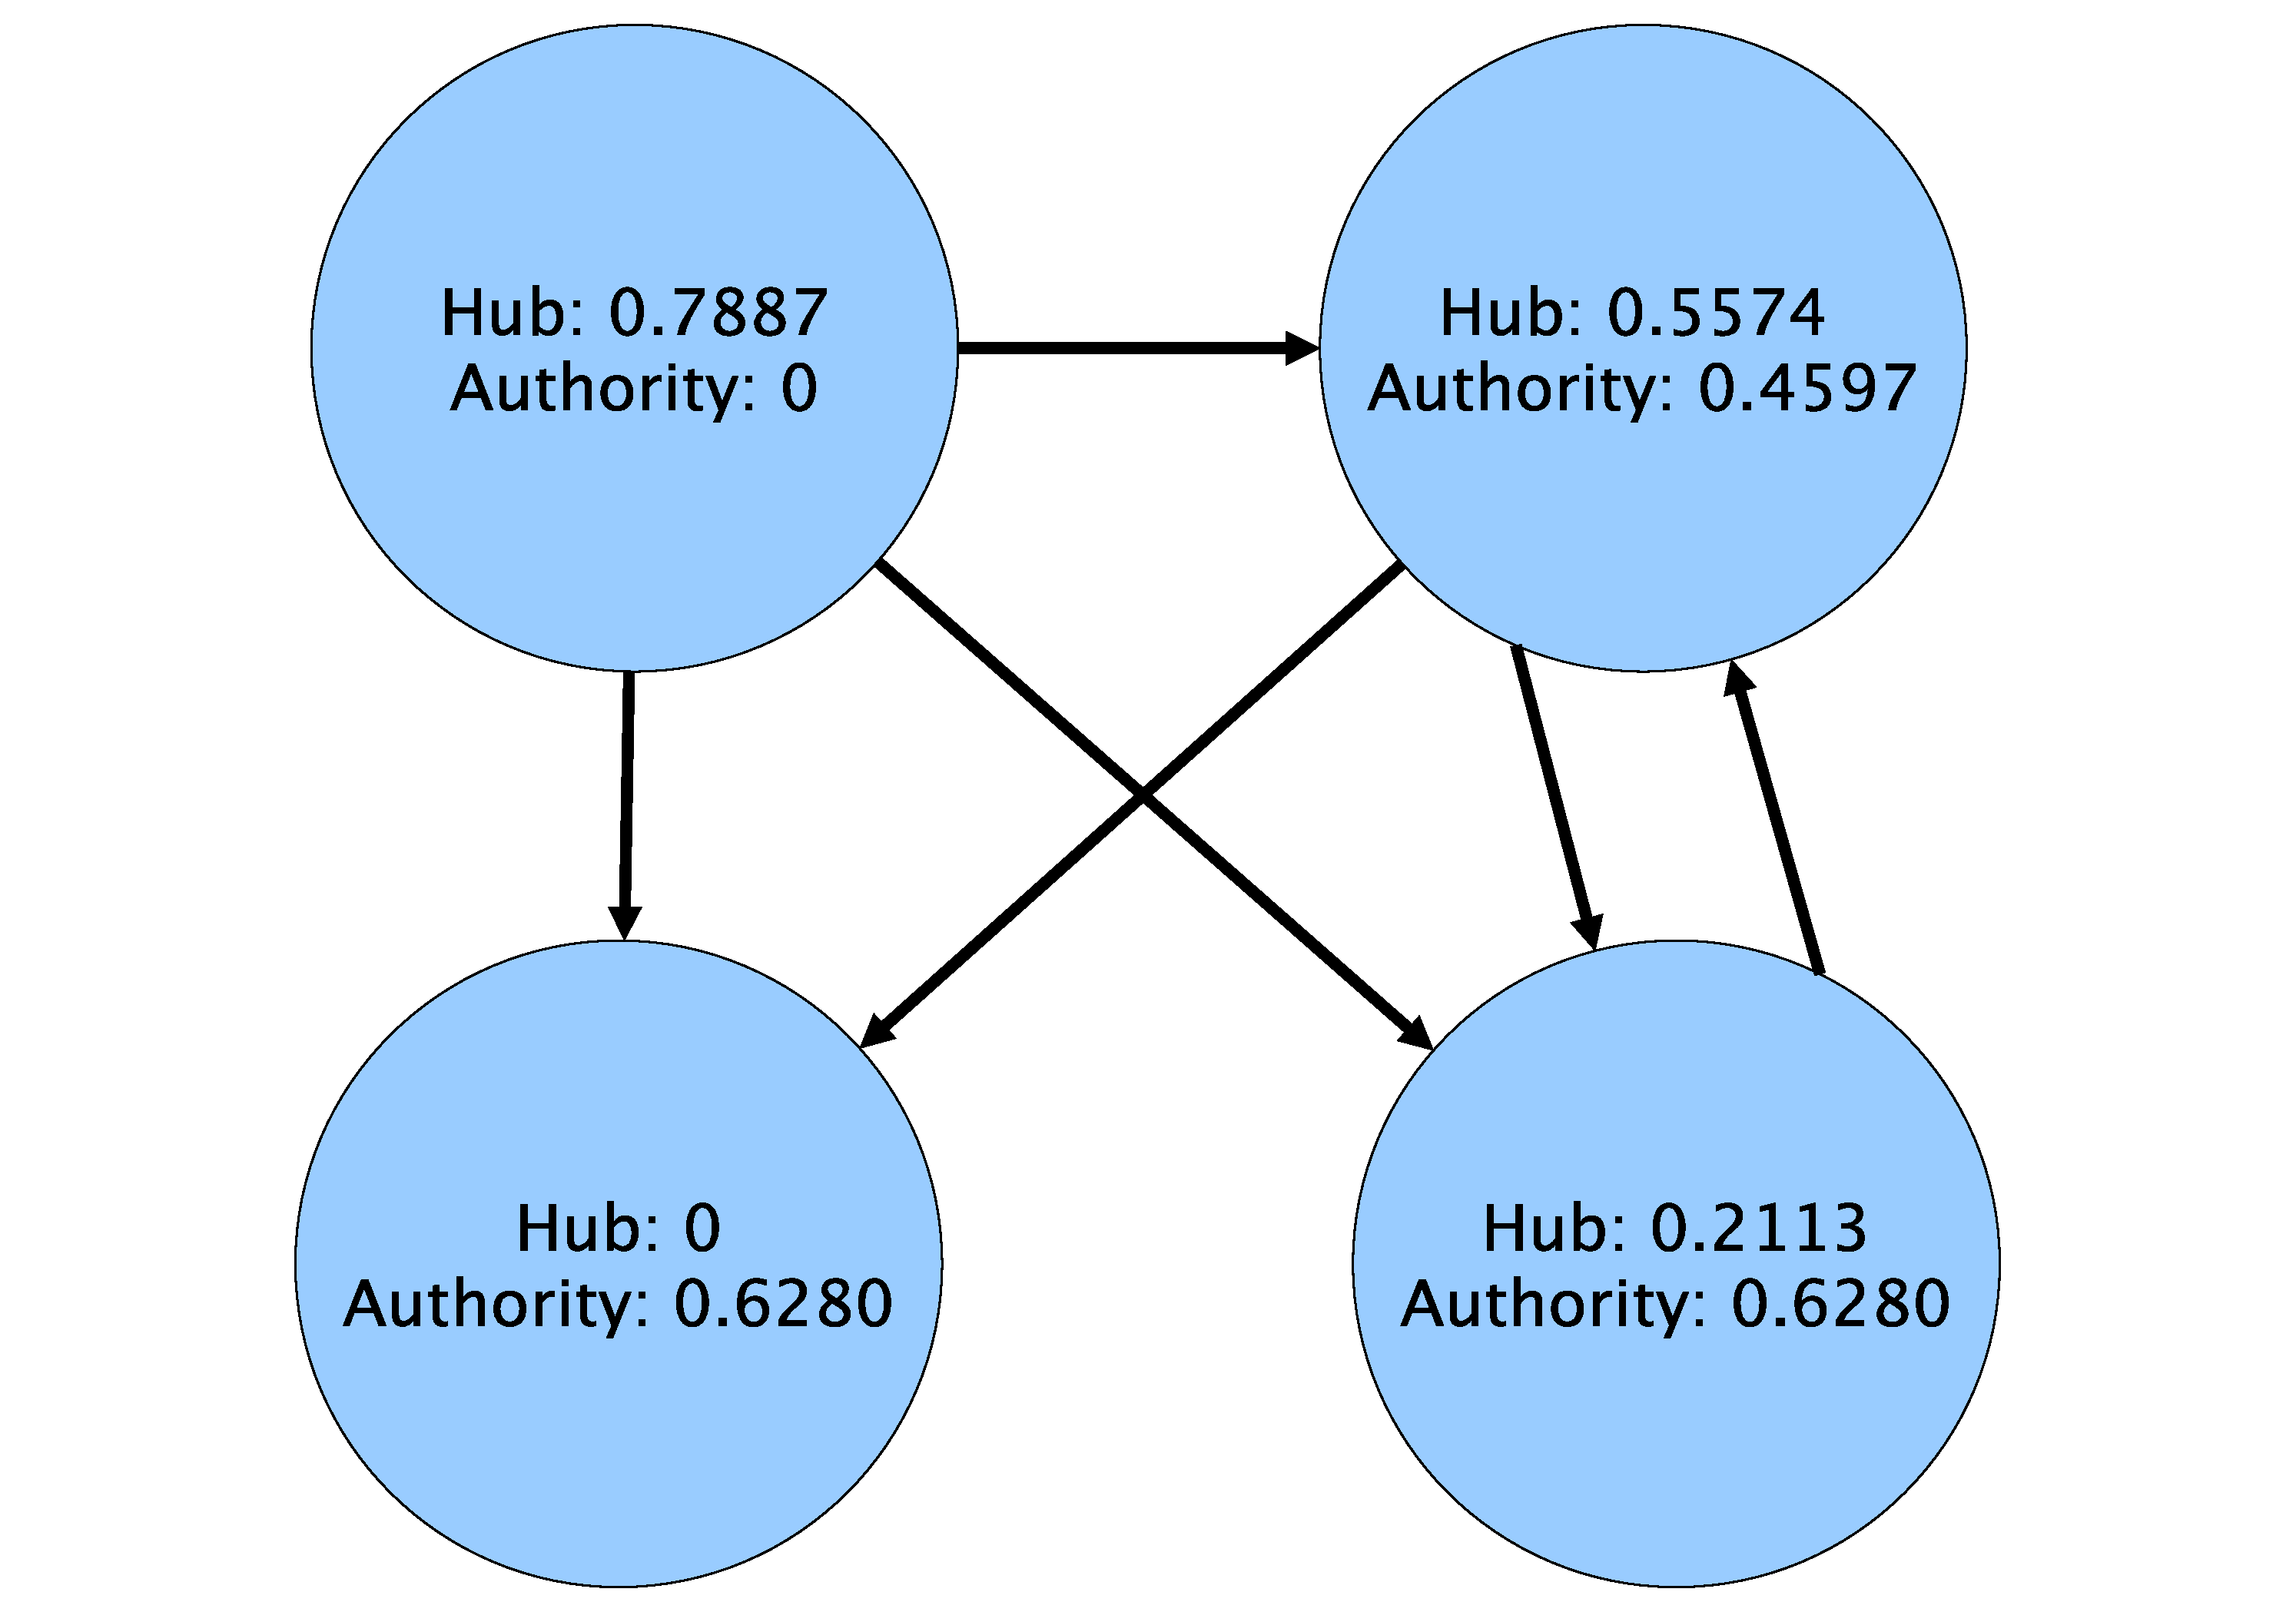
\includegraphics[width=0.5\textwidth]{figures/hits_example.pdf}
\caption{An example graph for HITS showing normalized hub and authority scores}
\label{hits:example}
\end{figure}

Hyperlink-Induced Topic Search (HITS)~\cite{hits} developed by Jon Kleinberg is
a link analysis algorithm that rates Web pages. The idea behind the algorithm is
to assign Hub and Authority scores to all vertices. Authorities are analagous to
web pages that have good authoritative content and get linked by other web pages.
Hubs can be thought of as large directories that themselves do not hold any
authoritative content but provide direct links to other authoritative pages.

HITS is an iterative algorithm where the Hub and Authority scores of vertices
from the previous iteration are used to compute the new scores. The
Hub and Authority scores of a vertex $v$, at the $i^{th}$ iteration, denoted by
$HUB(v_i)$ and $AUTHORITY(v_i)$ is computed as:
\begin{equation}
    \begin{aligned}
        AUTHORITY(v_i) = \sum_{u \in M(v)}({HUB(u_{i-1})})\\
        HUB(v_i) = \sum_{u \in M(v)}({AUTHORITY(v_{i})})
    \end{aligned}
\label{eq:hits}
\end{equation}

where $N$ is the number of vertices in the graph, $M(v)$ represents the set of
vertices that have an edge to vertex $v$, and $HUB(u_{i-1})$ and $AUTHORITY
(v_{i})$ represent the Hub score of vertex {u} in the $(i-1) ^{th}$ iteration and
Authority score of vertex $v$ in the $(i)^{th}$ iteration.

\subsection{Implementation Details} \label{sec:hits:implementation}

In this section, we discuss the MADlib implementation of HITS in depth.
We maintain two tables at every iteration: $message$ and $cur$. The
$cur$ table maintains the Hub and Authority scores of all vertices
computed in the previous iteration, while $message$ maintains the updated scores
of all vertices in the current iteration.

\begin{algorithm}[HITS$(V,E)$] \label{alg:hits:high}
\begin{algorithmic}[1]
	\State Create $cur$ table with a default Hub and Authority score of
			${1}$ for every vertex
	\Repeat
        \State Create empty table $message$.
        \State Update Authority score in $message$ using Hub scores of vertices
        in $cur$
        \State Update Hub score in $message$ using Authority scores of vertices
        in $message$
        \State Normalize Hub and Authority scores in $message$ using L2
        normalization
        \State Rename $message$ to $cur$
	\Until {both Authority and Hub scores have converged or \emph{max}
	iterations have elapsed}
\end{algorithmic}
\end{algorithm}

The following query is used to create and update the Hub and Authority scores
in $message$ table using the Hub scores in $cur$ table.

\begin{algorithm}[Update Hub and Authority scores$(cur, edge\_table)$]
\label{alg:hits:update}
\begin{lstlisting}
-- Create message table and update authority scores
CREATE TABLE message AS
	SELECT cur.id AS id,
		COALESCE(SUM(curalias.hub), 0.0) AS authority,
	cur.hub AS hub
	FROM cur
        LEFT JOIN edge_table ON cur.id = edge_table.dest
        LEFT JOIN cur AS curalias ON curalias.id = edge_table.dest
	GROUP BY cur.id, cur.hub
	ORDER BY cur.id

-- Update hub scores in message table:
UPDATE message
	SET hub = subquery.hub FROM
		(
		SELECT  message.id AS id, COALESCE(SUM(msgalias.authority), 0) AS hub
		FROM message
		LEFT JOIN edge_table ON message.id = edge_table.src
		LEFT JOIN message AS msgalias ON message.id = edge_table.dest
		GROUP BY  message.id
		) AS subquery
	WHERE subquery.id = message.id

\end{lstlisting}
\end{algorithm}


The Hub and Authority computations are terminated either when a fixed number of
iterations are completed, or when both the Hub and Authority scores of all
vertices have converged. The Hub/Authority score of a vertex is deemed
converged if the absolute difference in its Hub/Authority scores from $cur$ and
$message$ are less than a specified threshold.
The following query is used to find all the vertices whose Hub/Authority scores
have not converged yet.
\begin{algorithm}[Check for Hub and Authority convergence$(cur, message,
threshold)$]
\label{alg:hits:update1}
\begin{lstlisting}
		SELECT DISTINCT cur.id FROM message
		INNER JOIN cur ON cur.id=message.id
		WHERE ABS(cur.authority-message.authority) > threshold
		OR ABS(cur.hub-message.hub) > threshold
\end{lstlisting}
\end{algorithm}

\subsection{Best Practices} \label{sec:hits:bestpractices}

The HITS module in MADlib has a few optional parameters: number of iterations $max$,
and the threshold for convergence $threshold$.
The default values for these parameters when not specified by the user are $100$
and $\frac{1}{N*1000}$ respectively.
It is to be noted that this is not based on any experimental study. Users of
MADlib are encouraged to consider this factor when setting a value for threshold,
since a high $threshold$ value would lead to early termination of computation,
thus resulting in incorrect Hub and Authority scores.
